\section{Versuchsaufbau}

\begin{figure}[here]
\centering
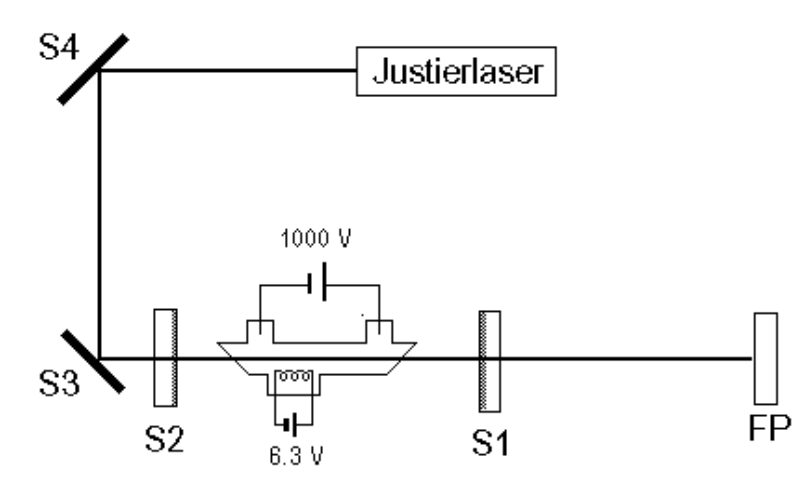
\includegraphics[scale=0.5]{img/HNL1}
\caption{Versuchsaufbau}
\begin{center}
\end{center}
\end{figure}

Der gesamte Versuchsaufbau ist in Abb. 7 schematisch dargestellt. Wir verwenden einen Justierlaser, zwei Umlenkspiegel (S3 und S4), zwei Resonatorspiegel (S1 und S2) und ein Scanning-Fabry-Perlot-Interferometer (FP, freier Spektralbereich = 2GHz). Zwischen S1 und S2 befindet sich unsere Gasentladungsröhre, die eine Heizspannung und eine Hochspannungsquelle zur Beschleunigung der Anregungselektronen benötigt. Außerdem werden wir ein Oszilloskop, einen Polarisator, verschiedene Linsen, einen Schirm, eine Irisblende und einen Bandpassfilter verwenden.